\subsection{Local Controller}
\label{sec:LocalController}

The local controller consists of a Proportional-Integral-Derivative Controller (PID) that receives as input a integer reference value (\emph{r}) from 0 to 1023, the LDR readings from 0 to 1023 (\emph{y}) and has as output the PWM duty cycle (\emph{u}) in the range 0 to 255.

The block diagram of the local controller is on Figure~\ref{fig:pid_block_diagram}. The error(\emph{e}) is defined as $e = r - y$. The signal \emph{u} is calculated as the sum of the proportional, integral and derivative components and the feedforward term.

\begin{figure}[!ht]
    \centering
        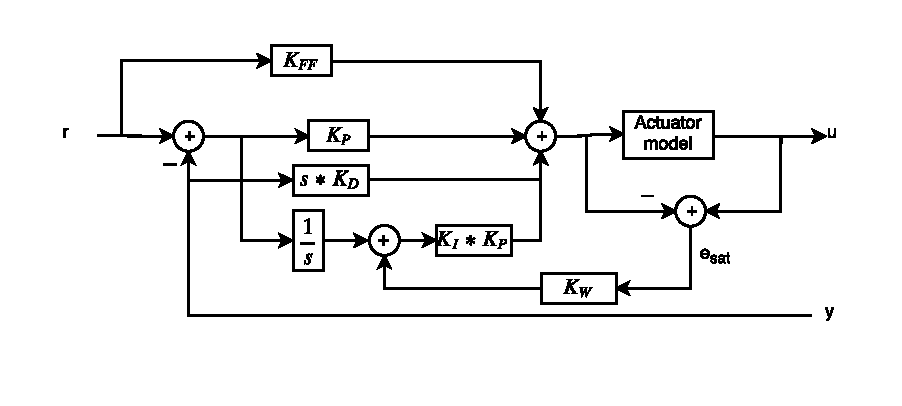
\includegraphics[scale=0.8]{img/pid_block_diagram}
    \caption{Local controller block diagram}\label{fig:pid_block_diagram}
\end{figure}


\subsubsection{Proportional Component}
\label{sub:ProportionalComponent}

The proportional component (\emph{P}) of the controller is just a gain multiplied (\emph{$K_p$}) by \emph{e}. $ P = K_p * e$.

\subsubsection{Integral Component}
\label{sub:IntegralComponent}

To approximate the integral of the error (\emph{I}) at sample \emph{k} we use the formula $ I_k = I_{k-1} + \frac{e_k-e_{k-1}}{2} * T_s$ .
We need to make this approximation as we don't have the continuous time values for the error.

\subsubsection{Derivative Component}
\label{sub:Derivative Component}

The derivative component (\emph{D}) is calculated as $ D = - K_d/T_s * (y_{k}-y_{k-1})$.
This component is calculated with signal \emph{y} instead of \emph{u} to avoid differentiating discontinuities, which would cause the signal \emph{u} to saturate.

\subsubsection{Anti-Windup}
\label{sub:AntiWindup}

The output of the integral component of the controller can be outside the range of values acceptable by the Arduino output.
This would lead the integrator to accumulate an error that would only disappear with the error being negative for multiple samples.
This causes a poor performance on the system.
To counter this effect we implemented a Anti-Windup block.
This block uses the difference between the expected controller output and the constrained value multiplied by a gain ($K_W$) to clean the integrator.

\subsubsection{Feedforward}
\label{sub:Feedforward}

The feedforward term(\emph{F}) depends only on the reference and is used to speed up the controller. It is calculated as $F = r * K_{FF}$, where $K_{FF}$ is the feedforward gain.

\subsubsection{Implementation Details}
\label{sub:Implementation Details}

The readings from the sensor are done with the average of three samples.

This controller was implemented as a interrupt routine to guarantee its execution in fixed intervals.

Todos os cálculos do controlador são feitos com valores de 0 a 1023, sendo convertidos quando necessário: para 0 a 255 para actuar o LED; e para lux quando são pedidos valores de iluminância.

\subsubsection{Parameters}
\label{sub:Parameters}

The gains of the controller were tuned by hand.
Following the guidelines from \emph{PID Without a PhD} \cite{PIDWhitoutPhD} we set the coarse values for each of them.
Then we a set of tests to both the step response and the incremental response we fined tuned the parameters.
The sampling time was chosen experimentally as the lowest value that allowed the rest of the code in the Arduino to exectude between each controller update.

The final values we use are:
\begin{description}
    \item[Proportional Gain] $K_P = 10$;
    \item[Derivative Gain] $K_D = 0.01$;
    \item[Integral Gain] $K_I = 10$;
    \item[Feedforward Gain] $K_FF = 0.1$;
    \item[Anti-Windup Gain] $K_W = 0.05$;
    \item[Sampling Time] $T_s = 1500 \mu s$;
\end{description}
